\section{Service Orchestration}
\rtext{Business Process:}
set of linked activities which realise business goal
\bluetext{Bus. Pro.} \redtext{vs} \greentext{Programs}
Granularity(Based on \bluetext{activities} \greentext{instructions}, 
Programming in \bluetext{large} \greentext{small}),
Control flow(\bluetext{Explicitly} \greentext{Implicitly} defined, 
\bluetext{Easy} \greentext{Not easy} understand),
\bluetext{Flexibility(change)},
\greentext{No Flexibility(Hard-coded)},
Execution(\bluetext{call third-party webservices}
\greentext{Invoke instructions locally},
, Scheduled by \bluetext{process engine} \greentext{OS})
%
\\
\rtext{BPEL, WS-BPEL:}
Web Services Business Process Execution Language(XML based),
to \orangetext{orchestrate loosely coupled services}
to model \bluetext{SOA's Business processe},
Def of business processes using web services at bus. proc. execution engine (ODE),
\orangetext{Lacks possibility} for formal verification compared to \greentext{FSP}
\redtext{Components:}
Activities,
State handling,
Control structures,
Exception handling,
Partner links,
Parallism,
Dead path elimination
\redtext{Related Standards:}
\bluetext{SOAP}
Simple Object Access Protocol,
Comm. platform in XML
\bluetext{WSDL}
Web Service Definition Language,
set of endpoints operating on Msg,
Operations and Msg described abstract, 
bound to concrete network protocol
\bluetext{UDDI}
Universal Description, Discovery and Integration,
Services registered, published, reused by other organizations,
App store for webservices
\\
\rtext{Service-Oriented Architecture SOA}
technique involving interaction between loosely coupled services 
that function independent;
modeled by \bluetext{WS-BPEL}.
\redtext{Principles:}
Loose coupling,
Service contract
$\rightarrow$
WSDL,
Abstraction of underlying logic,
Autonomy,
Reusability,
Composability $\rightarrow$ WS-BPEL,
Interoperability,
Discoverability $\rightarrow$ UDDI
\btext{BPMN vs BPEL}
Business friendly,
intuitive,
process oriented,
Swimlanes that represent organizational units,
User friendly data manipulations,
include human tasks,
expose web service UI
\redtext{VS}
technical,
manipulated with XPath expressions,
xpress orchestrations,
error handling,
compensating actions
\\
\redtext{Service composition}
\bluetext{conceptual model:}
S exchang Msg via out-port, in-port.
\bluetext{design methodology:}
\redtext{1Bottom-up:}
Serv. providers develop\& publish serv.;
Serv. consumers discover\&select serv.;
Serv. consumers compose selected serv..
\redtext{2Top-down:}
Serv. consumer develop global process;
Serv. consumers decompose global process into subprocess;
Serv. consumers select/develop services to implement subprocess.
\\
\redtext{Service orchestration}
\bluetext{Local perspective},
Describe control from one party‘s behavior(perspective),
\bluetext{WS-BPEL} as Standard,
Executable process which interact(Msg level) with web serv.
(Service internal / external),
Business process(business logic$+$task execution order,
span multiple apps and organizations,
Define long-lived TX multistep process model)
\\
\redtext{Service choreography}
Global perspective,
Describe global interactions among all the parties,
\bluetext{WS-CDL} as Standard
Tracks Msg sequences among multiple source and sinks,
Each involved party describes its part of the interaction
\bluetext{Orchest. vs Choreo.}
Two Orchest.(Web Service) sending each other(Choreo.)
\bluetext{Request, ACK, Accept, ACK}
\\
\rtext{Formal Methods:}
Modeling approaches, State machine verification,
(Finite state processes FSP, BPEL $\rightarrow$ LTS $\rightarrow$ FSP),
to represent and reason about \bluetext{Complexity of Concurrency Sy},
Performance optimization,
Deadlock detection, 
Dead Path elimination
\rtext{FSP}
Labeled Transition SY(
Abstract machine to study computation
Contains set of states and transitions between states)
\\
\bluetext{1.BPEL Basic Activitiy:
Receive,
Invoke,
Reply,
Assign,
Throw,
Exit,
Wait,
Empty.}:
Variable:
Global visibility <process>;
Visibility only within a <scope>.
<variables>
<variable name="coursename" type="xsd:string"/>
<variable name="grade" type="myNS:typeFromAnotherWSDL"/>
</variables>
\bluetext{2.BPEL Structured Activitiy:
Sequence,
If,
While Loop,
repeatUntil,
forEach,
Pick(Specifies which process executed check received event),
Flow,
Scop(exception).}
<while>
<condition>
\$iterations \&lt;3
</condition>
<invoke name="callSomeWebservice" ... />
</while>
\redtext{OR}
<forEach parallel="yes"counterName="N">
<startCounterValue>1</startCounterValue>
<finalCounterValue>5</finalCounterValue>
<scope>
<invoke name="callSomeWebservice"/>
</scope>
</forEach>
\rtext{BPEL$\rightarrow$FSP}
<invoke partner='p1' operation='o1'/>$\rightarrow$INVOKE = (invoke\_p1\_o1->END).
<receive partner='p2' operation='o2'/>$\rightarrow$RECEIVE = (receive\_p2\_o2->END).
<reply partner='p1' operation='o1'/>$\rightarrow$REPLY = (reply\_p1\_o->END).
\bluetext{Sequence}:
<sequence>
\begin{CJK*}{UTF8}{gbsn}
  \redtext{见上面BPEL三个}
\end{CJK*}
</sequence> 
$\rightarrow$
\begin{CJK*}{UTF8}{gbsn}
\redtext{见上面FSP三个}
\end{CJK*}
SEQUENCE = INVOKE; RECEIVE; REPLY; END. 
$0 \rightarrow 1\rightarrow 2 \rightarrow E$
\bluetext{Flow: Parallel Activity}
<flow>
\begin{CJK*}{UTF8}{gbsn}
\redtext{见上面BPEL三个}
\end{CJK*}
</flow>
$\rightarrow$
\begin{CJK*}{UTF8}{gbsn}
\redtext{见上面FSP三个}
\end{CJK*}
|| FLOW = (INVOKE || RECEIVE || REPLY).
$0 \rightarrow 1\rightarrow 2 \rightarrow E \leftarrow 4 \leftarrow 5 \leftarrow 6 \leftarrow 7$
\begin{CJK*}{UTF8}{gbsn}
\redtext{而且每点出3种Activity}
\end{CJK*}
\textbar
\rtext{\hlgray{Deadlock Detection}}:
\hlgray{when two or more competing activities are each waiting for the other to finish,}
\redtext{\hlgray{in FSP: a non-final-state with no outgoing arcs, like A sends to B, B sends to A}}
\bluetext{\hlgray{Assumption: Sync Comm}}
\hlgray{$!m_1$: Send a Msg of type m,
$?m_1$: Receive a Msg of type m}
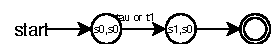
\includegraphics[width=\linewidth]{Deadlock_FSM.pdf}
\hlgray{$\tau$ for merge step}